\documentclass[12pt]{beamer}

\hypersetup{colorlinks=true,linkcolor=red}
\usetheme{default}
\usecolortheme{albatross}

\usepackage[utf8]{inputenc}
\usepackage[russian,english]{babel}
\usepackage[T2A]{fontenc}
\usepackage{hyperref}
\usepackage[final]{listings}
\usepackage{breakurl}
\usepackage{cite}
\usepackage{perpage}

\graphicspath{{img/}}

\def\Url\Breaks{\do\/\do-}
\lstset{
  frame=single,
  breaklines=true,
  basicstyle=\tiny,
  postbreak=\raisebox{0ex}{\ensuremath{\hookrightarrow\space}},
  numbers=left
}

\lstdefinestyle{base}{
  frame=single,
  breaklines=true,
  basicstyle=\tiny,
  postbreak=\raisebox{0ex}{\ensuremath{\hookrightarrow\space}},
  moredelim=[is][\color{red}]{-->}{<--},
  numbers=left
}

\MakePerPage{footnote}

\title{Operating Systems}
\subtitle{System calls and app loading}
\author{Me}
\date{\today}

\begin{document}
  \begin{frame}
    \titlepage
  \end{frame}

  \begin{frame}
\frametitle{Системные вызовы}
\begin{itemize}
  \item Системные вызовы - это механизм взаимодействия непривелигерованного кода
  (пользовательских приложений) и привелигированного кода (ядра)
  \begin{itemize}
    \item open/close, read/write, fork, exec и др. требуют обращения к ядру ОС.
  \end{itemize}
  \item Системный вызов осуществляет контролируемое повышение привелегий:
  \begin{itemize}
    \item нельзя дать произвольному коду выполняться в привелигированном режиме;
    \item при системном вызове вызывается определенная функция ядра ОС;
    \item функция ОС должна параноидально проверять все аргументы системного
    вызова на корректность.
  \end{itemize}
\end{itemize}
\end{frame}

\begin{frame}
\frametitle{Организация системных вызовов}
\begin{center}
  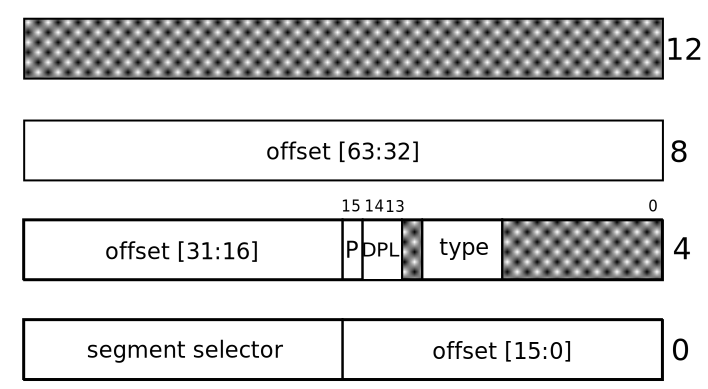
\includegraphics[width=.7\linewidth]{idt.png}
\end{center}
\begin{itemize}
  \item Типичный способ организации системного вызова - прерывания:
  \begin{itemize}
    \item например, в x86 можно использовать запись IDT с DPL равным 3;
    \item на практике используют специальные инструкции syscall/sysenter потому
    что они работают быстрее.
  \end{itemize}
\end{itemize}
\end{frame}

\begin{frame}
\frametitle{Передача аргументов и возврат значений}
\begin{itemize}
  \item При системном вызове типичным способом передачи аргументов и возврата
  значений являются регистры:
  \begin{itemize}
    \item например, в Linux Kernel используется следующая конвенция:
    \begin{itemize}
      \item регистр RAX соедржит номер системного вызова;
      \item регистры RDI, RSI, RDX, R10, R8, R9 содержат аргументы;
      \item результат возвращается в регистре RAX.
    \end{itemize}
  \end{itemize}
\end{itemize}
\end{frame}

\begin{frame}[fragile]
\frametitle{Пример: linux hello world}
\lstinputlisting{src/hello.S}
\end{frame}

\begin{frame}
\frametitle{Стек системного вызова}
\begin{itemize}
  \item Ядро оперирует данными всех приложений - не хочется, чтобы эти данные
  "утекали" в пространство пользователя:
  \begin{itemize}
    \item если обработчик системного вызова будет использовать стек приложения
    после возврата данные могут "утеч" в пространство пользователя;
    \item соответсвенно обработчик должен использовать другой стек, либо стек
    нужно "занулять" на выходе из системного вызова.
  \end{itemize}
\end{itemize}
\end{frame}

\begin{frame}
\frametitle{Стек системного вызова}
\begin{itemize}
  \item Ядро не знает размер стека пользовательского приложения:
  \begin{itemize}
    \item приложение могло использовать почти весь свой стек, и не оставить
    ничего ядру - мы не знаем, что приложение делало до системного вызова;
    \item т. е. для обработчика системного вызова, в конечном итоге, требуется
    свой стек, который выделяется ядром.
  \end{itemize}
\end{itemize}
\end{frame}

\begin{frame}
\frametitle{Task-State Segment (TSS)}
\begin{itemize}
  \item Task-State Segment - область памяти, в которой хранится информация о
  состоянии потока исполнения:
  \begin{itemize}
    \item в 32 битном x86 могла использоваться для аппаратного переключения
    контекста;
    \item в 64 битном x86 хранит указатель стека привилегированного режима
    \begin{itemize}
      \item при системном вызове/прерывании CPU загружает в RSP значения
      записанные в TSS перед вызовом обработчика.
    \end{itemize}
    \item структура TSS описана в разделе 7.7 Task Management in 64-bit Mode
    документации Intel.
  \end{itemize}
\end{itemize}
\end{frame}

\begin{frame}
\frametitle{Использование TSS}
\begin{itemize}
  \item Для использования TSS нужно выполнить две вещи:
  \begin{itemize}
    \item завести дескриптор в GDT описывающий TSS (формат дескриптора приведен
    в разделе 7.2.3 TSS Descriptor in 64-bit mode документации Intel);
    \item загрузить селектор этой записи в Task Register используя инструкцию
    LTR (раздел 7.2.4 Task Register документации Intel).
  \end{itemize}
\end{itemize}
\end{frame}

\begin{frame}
\frametitle{Соотношение TSS и потоков}
\begin{itemize}
  \item Похоже, изначально предполагалось использовать свою TSS для каждого
  потока
  \begin{itemize}
    \item гораздо проще завести по одной TSS на ядро, загрузить Task Register
    один раз для каждого ядра и при переключении потоков изменять
    непосредственно TSS;
    \item таким образом получается, что у каждого потока есть два стека: стек
    пространства ядра и стек пространcтва пользователя (если поток вообще
    работает в пространстве пользователя).
  \end{itemize}
\end{itemize}
\end{frame}

  \begin{frame}
\frametitle{Исполняемые файлы}
\begin{itemize}
  \item Ядро ОС само по себе не очень полезно - пользователи имеют дело с
  прикладными приложениями
  \begin{itemize}
    \item соответственно, для полноценной ОС желательно уметь загружать и
    запускать программы.
  \end{itemize}
  \item Программы представляются как один или несколько исполняемых файлов:
  \begin{itemize}
    \item скрипты с аттрибутом +x и \#\! в начала файла;
    \item ELF файлы (опять же с аттрибутом +x);
    \item PE/COM файлы (это в Windows);
    \item Mach-O (это в Mac OS).
  \end{itemize}
\end{itemize}
\end{frame}

\begin{frame}
\frametitle{Бинарные исполняемые файлы}
\begin{itemize}
  \item Бинарный исполняемый файл содержит:
  \begin{itemize}
    \item код и данные необходимые для выполнения;
    \item ссылки на другие бинарные файлы (разделяемые библиотеки);
    \item может содержать отладочную информацию.
  \end{itemize}
  \item Бинарный исполняемый файл определяет
  \begin{itemize}
    \item где в памяти должны располагаться данные и код;
    \item где находится точка входа в программу (условно, адрес main).
  \end{itemize}
\end{itemize}
\end{frame}

\begin{frame}[fragile]
\frametitle{Формат ELF}
\begin{columns}
  \begin{column}{.36\linewidth}
    \begin{lstlisting}
struct elf_hdr {
    uint8_t e_ident[ELF_NIDENT];
    uint16_t e_type;
    uint16_t e_machine;
    uint32_t e_version;
    uint64_t e_entry;
    uint64_t e_phoff;
    uint64_t e_shoff;
    uint32_t e_flags;
    uint16_t e_ehsize;
    uint16_t e_phentsize;
    uint16_t e_phnum;
    uint16_t e_shentsize;
    uint16_t e_shnum;
    uint16_t e_shstrndx;
} __attribute__((packed));
    \end{lstlisting}
  \end{column}
  \begin{column}{.65\linewidth}
    \begin{itemize}
      \item ELF файл начинается с заголовка с общей информацией;
      \item тип, версия, архитектура - ОС должна проверить файл на валидность;
      \item адрес точки входа так же хранится здесь - \emph{e\_entry}.
    \end{itemize}
  \end{column}
\end{columns}
\end{frame}

\begin{frame}
\frametitle{Program Header}
\begin{itemize}
  \item Program Header, упрощенно, описывает участок памяти который должна
  подготовить ОС
  \begin{itemize}
    \item все Program Header-ы хранятся в таблице в ELF файле;
    \item при загрузке ELF файла, ОС должна прочитать эту таблицу и подготовить
    участки памяти.
  \end{itemize}
  \item Таблица Program Header-ов:
  \begin{itemize}
    \item смещение таблицы в файле хранится в поле \emph{e\_phoff};
    \item количество записей в таблице хранится в поле \emph{e\_phnum};
    \item размер каждой записи хранится в поле \emph{e\_phentsize}.
  \end{itemize}
\end{itemize}
\end{frame}

\begin{frame}[fragile]
\frametitle{Program Header для x86}
\begin{columns}
  \begin{column}{.65\linewidth}
    \begin{itemize}
      \item \emph{p\_type} - тип заголовка (на интересует только
      \emph{PT\_LOAD} == 1);
      \item \emph{p\_vaddr} и \emph{p\_memsz} - адрес и размер в памяти;
      \item \emph{p\_offset} и \emph{p\_filesz} - смещение и размер в файле
      данных, которые нужно загрузить в память;
      \item \emph{p\_filesz} может быть меньше \emph{p\_memsz}, хвост должен
      быть заполнен нулями.
    \end{itemize}
  \end{column}
  \begin{column}{.36\linewidth}
    \begin{lstlisting}
struct elf_phdr {
    uint32_t p_type;
    uint32_t p_flags;
    uint64_t p_offset;
    uint64_t p_vaddr;
    uint64_t p_paddr;
    uint64_t p_filesz;
    uint64_t p_memsz;
    uint64_t p_align;
} __attribute__((packed));
    \end{lstlisting}
  \end{column}
\end{columns}
\end{frame}

\begin{frame}
\frametitle{Загрузка ELF файла}
\begin{itemize}
  \item Таким образом загрузка ELF файла в простом случае состоит из следующих
  действий:
  \begin{itemize}
    \item проверяем заголовок ELF файла - что это ELF файл для нужной
    архитектуры;
    \item читаем таблицу Program Header-ов аллоцируем память и подготавливаем
    таблицу страниц для всех Program Header-ов с типом \emph{PT\_LOAD};
    \item передаем управление точке входа с переключением процессора в
    непривелигированный режим работы.
  \end{itemize}
\end{itemize}
\end{frame}

  \begin{frame}
\frametitle{Библиотеки}
\begin{itemize}
  \item Библиотеки позволяют переиспользовать код (зачастую без перекомпиляции):
  \begin{itemize}
    \item библиотеки можно организовывать разными способами, например:
    \begin{itemize}
      \item статические библиотеки - просто наборы объектных файлов, которые
      можно слинковать с вашей программой;
      \item динамические библиотеки подключаются во время работы программы.
    \end{itemize}
  \end{itemize}
  \item Преимущества динамических библиотек:
  \begin{itemize}
    \item не нужно хранить один и тот же код в нескольких экземплярах (в отличие
    от статических библиотек);
    \item можно избежать дублирования одного и того же кода в памяти (загрузить
    динамическую библиотеку в единственном экземпляре на все программы).
  \end{itemize}
\end{itemize}
\end{frame}

\begin{frame}
\frametitle{Динамические библиотеки}
\begin{itemize}
  \item Динамическая библиотека может быть загружена по любому адресу:
  \begin{itemize}
    \item почему мы не можем зафиксировать адрес?
    \item исполняемый файл не может заранее знать адреса функций и данных из
    библиотеки;
    \item сама библиотека не может знать адреса своих функций и данных заранее.
  \end{itemize}
\end{itemize}
\end{frame}

\begin{frame}
\frametitle{Position Independent Code (PIC)}
\begin{itemize}
  \item В момент сборки мы можем не знать абсолютные адреса функций/переменных,
  но мы можем знать относительные:
  \begin{itemize}
    \item функция которую мы хотим вызвать находится на \emph{x} байт выше/ниже
    текущей инструкции (значения регистра RIP);
    \item аналогично для данных.
  \end{itemize}
  \item PIC решает проблему обращения к функциям и переменным внутри
  динамической библиотеки
  \begin{itemize}
    \item если библиотека зависит от другой библиотеки - у нас все еще проблемы;
    \item программам/библиотекам зависящим от нас это не помогает.
  \end{itemize}
\end{itemize}
\end{frame}

\begin{frame}
\frametitle{Динамический компоновщик}
\begin{itemize}
  \item Динамический компоновщик решает ту же задачу, что и обычнй, но в других
  условиях
  \begin{itemize}
    \item в ELF файле может быть специальный Program Header с типом
    \emph{PT\_INTERP == 3} - он указывает на путь к динамическому компоновщику;
    \item вместе с имполняемым файлом ОС загружает динамический компоновщик
    \emph{и передает ему управление}.
  \end{itemize}
  \item Динамический компоновщик загружает нужные динамические библиотеки
  \begin{itemize}
    \item информация о необходимых библиотеках хранится в месте, на которое
    указывает Program Header \emph{PT\_DYNAMIC};
    \item т. е. в момент сборки мы должны знать обо всех библиотеках, от
    которых мы зависим.
  \end{itemize}
\end{itemize}
\end{frame}

\begin{frame}
\frametitle{Редактирование связей}
\begin{itemize}
  \item Динамический компоновщик нашел и загрузил все библиотеки в память, что
  дальше?
  \begin{itemize}
    \item теперь ему известны адреса всех нужных функций и переменных;
    \item он может подредактировать память и проставить в нужных местах ссылки.
  \end{itemize}
  \item Нужное место - Global Offset Table (GOT):
  \begin{itemize}
    \item по сути, таблица адресов всех объектов, к которым нам нужно
    обращаться;
    \item динамический компоновщик зная адреса просто заполняет GOT.
  \end{itemize}
\end{itemize}
\end{frame}

\begin{frame}[fragile]
\frametitle{Пример}
\begin{columns}
  \begin{column}{.3\linewidth}
    \begin{lstlisting}
int bar;

void foo(void)
{ ++bar; }
    \end{lstlisting}
  \end{column}
  \begin{column}{.6\linewidth}
    \begin{lstlisting}[style=base]
foo:
  push   %rbp
  mov    %rsp,%rbp

  -->mov    0x20093d(%rip),%rax // 0x200fd8<--
  -->mov    (%rax),%eax<--
  lea    0x1(%rax),%edx
  mov    0x200931(%rip),%rax
  mov    %edx,(%rax)

  nop
  pop    %rbp
  retq 
    \end{lstlisting}
  \end{column}
\end{columns}
\end{frame}

\begin{frame}[fragile]
\frametitle{Пример}
\begin{itemize}
  \item Куда указывает \emph{0x200fd8}? Посмотрим с помощью \emph{readelf -S}:
  \begin{lstlisting}
[Nr] Name Type     Address Offset Size EntSize Flags Link Info Align
...
[19] .got PROGBITS 200fd0  fd0    30   8       WA    0    0    8
...
  \end{lstlisting}
  \begin{itemize}
    \item динамический компоновщик после загрузки libfoo.so запишет в нужное
    место .got адрес переменной bar;
    \item а адрес .got находится с помощью относительной адресации.
  \end{itemize}
\end{itemize}
\end{frame}

\begin{frame}[fragile]
\frametitle{Пример}
\begin{columns}
  \begin{column}{.5\linewidth}
    \begin{lstlisting}[style=base]
main:
  push   %rbp
  mov    %rsp,%rbp

  mov    0x200930(%rip),%eax
  mov    %eax,%esi
  mov    $0x4007d4,%edi
  mov    $0x0,%eax
  callq  4005d0 <printf@plt>

  -->callq  4005f0 <foo@plt><--

  mov    0x200914(%rip),%eax
  mov    %eax,%esi
  mov    $0x4007e6,%edi
  mov    $0x0,%eax
  callq  4005d0 <printf@plt>

  mov    $0x0,%eax
  pop    %rbp
  retq
    \end{lstlisting}
  \end{column}
  \begin{column}{.4\linewidth}
    \begin{lstlisting}
int main(void)
{
  printf("bar = %d\n", bar);
  foo();
  printf("bar = %d\n", bar);
  return 0;
}
    \end{lstlisting}
  \end{column}
\end{columns}
\end{frame}

\begin{frame}[fragile]
\frametitle{Пример}
\begin{itemize}
  \item Что за функция \emph{foo@plt}?
\begin{lstlisting}
foo@plt:
  jmpq   *0x200a32(%rip) // 0x601028
  pushq  $0x2
  jmpq   4005c0 <_init+0x20>
\end{lstlisting}
  \begin{itemize}
    \item адрес \emph{0x601028} просто ссылается на определенное место в got;
    \item т. е. foo@plt просто передает управление по адресу записанному в got;
    \item в конечном итоге, там должен оказаться адрес функции foo.
  \end{itemize}
\end{itemize}
\end{frame}


  \begin{frame}
  \begin{center}
  \Huge Q\&A
  \end{center}
  \end{frame}
\end{document}
